\documentclass[../main.tex]{subfiles}
\graphicspath{{figures/}{../figures/}}

\begin{document}
% \todo[color=green!40]{完成问题三模型的求解(sections/q3\_solution)}

通过模拟物理退火过程的随机搜索与概率接受机制,在多无人机、多烟幕弹的决策变量可行域内寻找使有效遮蔽时间$\Delta t$最大化的最优解,具体步骤如下:

\noindent\textbf{步骤1 初始化参数}
\begin{itemize}
    \item \textbf{初始解生成}:在决策变量可行域内随机生成初始解$S_0=\{\alpha_j, v_{\text{FYj}}, t_{\text{FYj},i1}, t_{\text{FYj},i2}\}$($j=1,2,\dots,5$为无人机编号,$i=1,2,3$为烟幕弹编号),确保满足时间约束(如$t_{\text{FYj},(i+1)1} \geq t_{\text{FYj},i1}+1$、$t_{\text{FYj},i2} \geq t_{\text{FYj},i1}$);
    \item \textbf{初始温度$T_0$}:设定较高的初始温度(如$T_0=100$),确保算法初期能接受较差解,扩大对多变量组合的搜索范围;
    \item \textbf{降温系数$k$}:设定降温速率(如$k=0.95$),控制温度随迭代逐步降低,平衡全局探索与局部精细搜索;
    \item \textbf{终止温度$T_{\text{end}}$}:设定停止阈值(如$T_{\text{end}}=10^{-5}$),当温度低于此值时,算法收敛,终止迭代;
    \item \textbf{迭代次数$L$}:设定每轮温度下的迭代步数(如$L=100$),确保在当前温度下对邻域解进行充分搜索,避免遗漏较优解。
\end{itemize}

\noindent\textbf{步骤2 目标函数计算(核心步骤)}

对任意解$S=\{\alpha_j, v_{\text{FYj}}, t_{\text{FYj},i1}, t_{\text{FYj},i2}\}$,计算其对应的有效遮蔽时间$\Delta t$,步骤如下:
\begin{itemize}
\item \textbf{多轨迹同步模拟}:

导弹$Mk$轨迹:按位置公式计算任意时刻$t$的坐标$(x_{\text{Mk},t}, y_{\text{Mk},t}, z_{\text{Mk},t})$,即沿指向假目标的直线飞行;

无人机$FYj$轨迹:根据$\alpha_j$和$v_{\text{FYj}}$,计算投放时刻$t_{\text{FYj},i1}$的位置$(x_{\text{FYj},t_{\text{FYj},i1}}, y_{\text{FYj},t_{\text{FYj},i1}}, z_{\text{FYj},t_{\text{FYj},i1}})$,保持$z$轴高度不变;

烟幕弹起爆轨迹:基于$t_{\text{FYj},i2} - t_{\text{FYj},i1}$的时间差,计算起爆位置$(x_{\text{FYji},t_{\text{FYj},i2}}, y_{\text{FYji},t_{\text{FYj},i2}}, z_{\text{FYji},t_{\text{FYj},i2}})$,$x,y$方向随无人机惯性运动,$z$方向受重力下落;

烟幕云团轨迹:对$t \in [t_{\text{FYj},i2}, t_{\text{FYj},i2}+\Delta t_0]$($\Delta t_0$为烟幕有效时长),计算云团中心坐标$(x_{\text{FYji},t}, y_{\text{FYji},t}, z_{\text{FYji},t})$,$x,y$坐标恒定,$z$方向以$v_1$匀速下沉;
\item \textbf{真目标采样}:在真目标圆柱面($x_1^2+(y_1-y_0)^2=r_0^2$,$z_1 \in [0,h_0]$)上均匀采样(如10个角度×5个高度,共50个采样点),覆盖目标所有关键区域;
\item \textbf{遮挡时间判定}:对每个采样点和每个时间$t$,判断是否被任一烟幕云团球体($O_{\text{FYji},t}: (x-x_{\text{FYji},t})^2+(y-y_{\text{FYji},t})^2+(z-z_{\text{FYji},t})^2=r^2$)遮挡,若满足$\sum_{j=1}^5\sum_{i=1}^3 a_i^j \neq 0$($a_i^j$为遮挡标识,1表示遮挡,0表示未遮挡),则记录$t$为遮挡时刻;
\item \textbf{有效时长统计}:合并所有连续的遮挡时间区间,计算总时长,即为该解对应的$\Delta t$。
\end{itemize}

\noindent\textbf{步骤3 邻域解生成}

为当前解$S=\{\alpha_j, v_{\text{FYj}}, t_{\text{FYj},i1}, t_{\text{FYj},i2}\}$生成邻域解$S'$,确保新解满足所有约束条件:
\begin{itemize}
\item 方向角$\alpha_j'$:$\alpha_j' = \alpha_j + \Delta\alpha$,其中$\Delta\alpha$为$[-0.1,0.1]$弧度的随机扰动,若$\alpha_j'$超出$[0,2\pi]$,则通过取模($\alpha_j' = \alpha_j' \mod 2\pi$)调整至可行域;
\item 飞行速度$v_{\text{FYj}}'$:$v_{\text{FYj}}' = v_{\text{FYj}} + \Delta v$,其中$\Delta v$为$[-3,3]$ m/s的随机扰动,若$v_{\text{FYj}}'$超出$[70,140]$ m/s,则截断至边界(小于70取70,大于140取140);
\item 投放时刻$t_{\text{FYj},i1}'$:$t_{\text{FYj},i1}' = t_{\text{FYj},i1} + \Delta t$,其中$\Delta t$为$[-0.3,0.3]$ s的随机扰动,调整后需满足$t_{\text{FYj},(i+1)1}' \geq t_{\text{FYj},i1}'+1$及$t_{\text{FYj},i1}' \in [0, d_{\text{mk},0}/v_0]$($d_{\text{mk},0}$为导弹初始距离假目标的距离);
\item 起爆时刻$t_{\text{FYj},i2}'$:$t_{\text{FYj},i2}' = t_{\text{FYj},i2} + \Delta t$,其中$\Delta t$为$[-0.3,0.3]$ s的随机扰动,调整后需满足$t_{\text{FYj},i2}' \geq t_{\text{FYj},i1}'$及$t_{\text{FYj},i2}' \in [t_{\text{FYj},i1}', d_{\text{mk},0}/v_0]$。
\end{itemize}

\noindent\textbf{步骤4 判断准则(接受/拒绝新解)}
\begin{itemize}
\item 计算目标函数差值:$\Delta E = \Delta t(S') - \Delta t(S)$,其中$\Delta t(S')$为邻域解的有效遮蔽时间,$\Delta t(S)$为当前解的有效遮蔽时间;
\item 若$\Delta E > 0$(新解更优):直接接受$S'$作为当前解,更新当前解的参数与$\Delta t$;
\item 若$\Delta E \leq 0$(新解较差):以概率$P = \exp\left(\frac{\Delta E}{T}\right)$接受$S'$($T$为当前温度),通过生成$[0,1]$区间的随机数$rand$,若$rand < P$,则接受$S'$,否则保留原解。温度越高,$P$越大,越容易接受较差解,利于跳出局部最优。
\end{itemize}

\noindent\textbf{步骤5 降温与迭代}
\begin{itemize}
\item 每完成$L$次迭代(即对当前温度下的$L$个邻域解完成接受/拒绝判断)后,按$T = k \cdot T$降低温度,逐步减小对较差解的接受概率;
\item 重复“邻域解生成→接受/拒绝判断→降温”的循环过程,直至当前温度$T \leq T_{\text{end}}$,停止迭代。
\end{itemize}

\noindent\textbf{步骤6 终止与最优解输出}

迭代终止后,从所有历史解中筛选出有效遮蔽时间$\Delta t$最大的解,作为最优解$S^*=\{\alpha_j^*, v_{\text{FYj}}^*, t_{\text{FYj},i1}^*, t_{\text{FYj},i2}^*\}$,并输出$S^*$的所有参数及对应的最大有效遮蔽时间$\Delta t^*$。





\begin{table}[H]
\caption{标准三线表格}
\label{tab:001} 
\centering
\begin{small}
\begin{tabular}{cccc}
\toprule[1.5pt]
无人机编号 &无人机运动方向 & 无人机运动速度  &烟幕干扰弹编号     \\  
\midrule[1pt]
  FY1           &7.45                   & 72.00     & 1     \\               
   FY1          &7.45                  & 72.00     & 2      \\               
   FY1          &7.45                   & 72.00     & 3    \\                
  FY2           &295.07                   & 127.02     & 1      \\                
  FY2           &295.07                   & 127.02     & 2       \\               
  FY2           &295.07                   & 127.02    & 3     \\               
  FY3           & 79.64                  & 82.34     & 1       \\               
FY3             & 79.64                  & 82.34     & 2    \\                
FY3             & 79.64                  & 82.34    & 3      \\                
  FY4           &0                   & 70.00     & 1      \\                
  FY4           &0                   & 70.00     & 2       \\               
  FY4           &0                   & 70.00    & 3     \\               
  FY5          & 120.32                 & 104.78     & 1       \\               
FY5         & 120.32                 & 104.78    & 2    \\                
FY5          &120.32                  & 104.78     & 3      \\               
\bottomrule[1.5pt]
\end{tabular}
\end{small}
\end{table}


\begin{table}[H]
\caption{标准三线表格}
\label{tab:031} 
\centering
\begin{small}
\begin{tabular}{cccc}
\toprule[1.5pt]
烟幕干扰弹投放点的x坐标& 烟幕干扰弹投放点的y坐标    &烟幕干扰弹投放点的z坐标 & 烟幕干扰弹起爆点的x坐标\\
\midrule[1pt]
    17800.71 & 0.09    & 1800.00 & 17801.43 \\
    17871.39 & 9.33    & 1800.00 & 17903.52 \\
    19121.47 & 172.77  & 1800.00 & 19180.73 \\
    12425.24 & 491.10  & 1400.00 & 12457.54 \\
    12707.30 & -111.76 & 1400.00 & 12851.56 \\
    13363.47 & -1514.23& 1400.00 & 13757.49 \\
    6501.92  & -254.17 & 700.00  & 6509.32 \\
    6516.87  & -172.36 & 700.00  & 6555.07 \\
    6531.68  & -91.36  & 700.00  & 6564.69 \\
    11064.40 & 2000.00 & 1800.00 & 11099.40 \\
    11134.40 & 2000.00 & 1800.00 & 11228.20 \\
    11204.40 & 2000.00 & 1800.00 & 11239.40 \\
    12151.52 & -549.23 & 1300.00 & 11821.44 \\
    12069.53 & -409.04 & 1300.00 & 11821.4 \\
    11858.99 & -49.06  & 1300.00 & 11759.02 \\
\bottomrule[1.5pt]
\end{tabular}
\end{small}
\end{table}




\begin{table}[H]
\caption{标准三线表格}
\label{tab:031} 
\centering
\begin{small}
\begin{tabular}{cccc}
\toprule[1.5pt]
干扰弹起爆点的y坐标&干扰弹起爆点的z坐标&有效干扰时长 &干扰的导弹编号\\
\midrule[1pt]
0.19    & 1800.00 & 2.64 & M1 \\
    13.53   & 1799.01 & 4.50 & M1 \\
    180.51  & 1796.62 & 0    & 0 \\
    422.07  & 1398.24 & 4.09 & M2 \\
    -420.10 & 1364.81 & 3.38 & M3 \\
    -2356.40& 1137.45 & 0    & 0 \\
    -213.67 & 698.77  & 1.57 & M3 \\
    36.61   & 667.38  & 2.90 & M1 \\
    89.26   & 675.63  & 0    & 0 \\
    2000.00 & 1798.78 & 0    & 0 \\
    2000.00 & 1791.20 & 0    & 0 \\
    2000.00 & 1798.78 & 0    & 0 \\
    -399.99 & 1286.66 & 1.04 & M3 \\
    15.16   & 1192.22 & 3.51 & M1 \\
    121.89  & 1282.50 & 0    & 0 \\             
\bottomrule[1.5pt]
\end{tabular}
\end{small}
\end{table}
\begin{figure}[H]
\centering
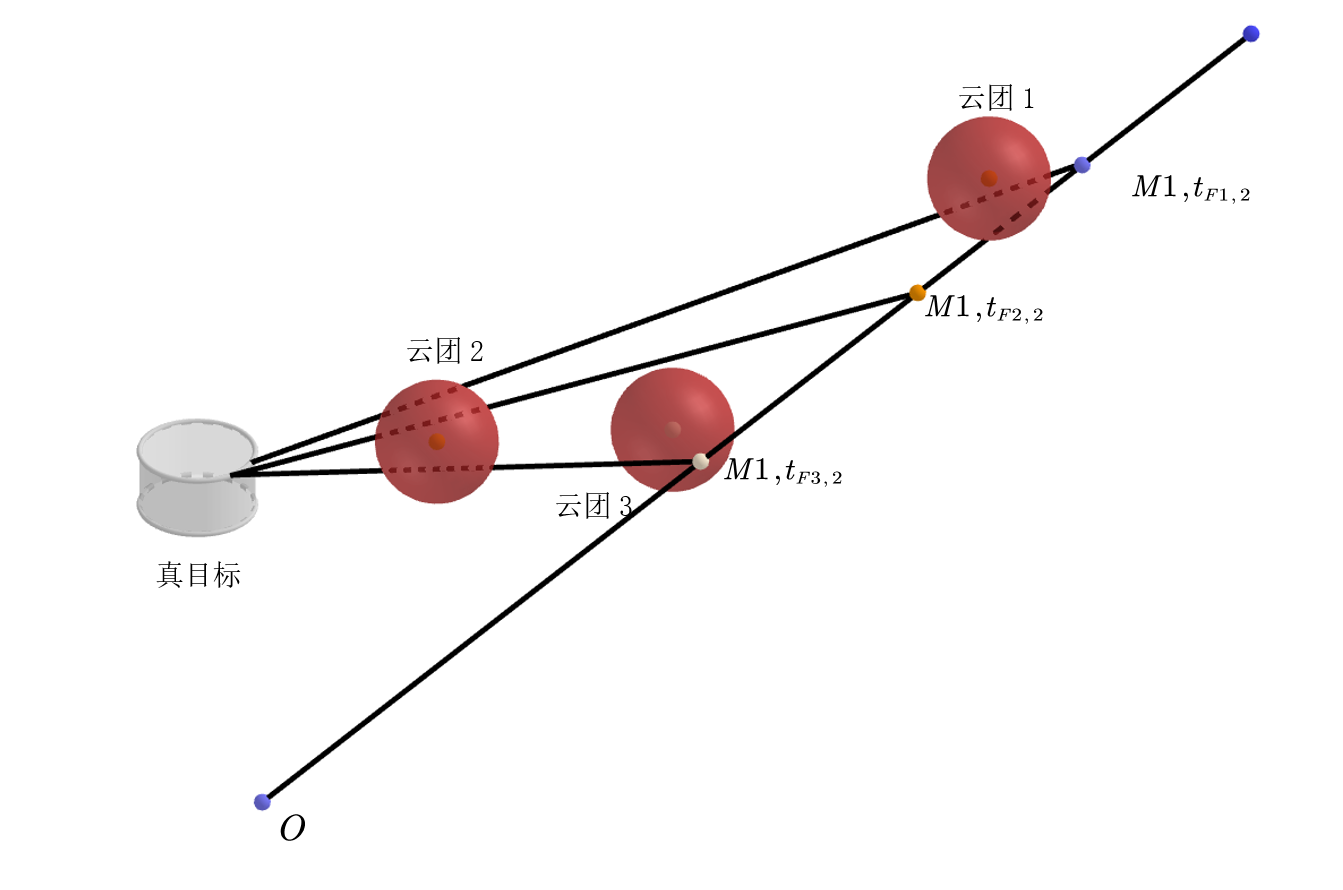
\includegraphics[scale=0.5]{图三.png}
\caption{}
\label{图3}
\end{figure}



\end{document}